\documentclass[11pt]{article}
\usepackage[margin=1in]{geometry}
\usepackage{amsmath,amssymb,amsthm}
\usepackage{booktabs}
\usepackage{enumitem}
\usepackage{tikz}
\usetikzlibrary{arrows.meta}
\usepackage{hyperref}
\hypersetup{colorlinks=true,linkcolor=blue,urlcolor=blue,citecolor=blue}

\theoremstyle{plain}
\newtheorem{theorem}{Theorem}
\newtheorem{lemma}[theorem]{Lemma}
\newtheorem{proposition}[theorem]{Proposition}
\newtheorem{corollary}[theorem]{Corollary}
\newtheorem{conjecture}[theorem]{Conjecture}
\theoremstyle{definition}
\newtheorem{definition}[theorem]{Definition}
\theoremstyle{remark}
\newtheorem*{remark}{Remark}
\setlength{\parskip}{0.45em}

\title{The kernel method on odd toroidal grids}
\author{Siddharth Narayan Mishra \\ \small working draft of a section for the joint $C_3\square C_n$ paper}
\date{October 26, 2026}

\begin{document}
\maketitle

\begin{abstract}
For odd $m,n$ the Alon--Tarsi number of $C_m\square C_n$ is $4$, so the polynomial
method cannot prove 3-choosability. We examine the other standard tool, the kernel
method of Bondy--Boppana--Siegel and Galvin. For $m=3$ we settle it completely: for odd
$n$, $C_3\square C_n$ has a kernel-perfect orientation with maximum out-degree $2$ if and
only if $3\mid n$, and then there are exactly $12$ of them. The ``only if'' direction has
a hand proof: every other orientation contains an explicit induced odd directed cycle.
The ``if'' direction is a finite computer-assisted proof valid for all $n$. For $m=5$ the
method fails already on $C_5\square C_5$. So the kernel method recovers 3-choosability of
$C_3\square C_n$ exactly when $3\mid n$, which explains why a different method is needed.
\end{abstract}

\section{Setting}

$G=C_3\square C_n$, $n$ odd. Vertex $(r,c)$ has row $r\in\mathbb Z_3$ and column
$c\in\mathbb Z_n$. Each column is a triangle, each row an $n$-cycle. A \emph{kernel} of a
digraph is an independent set $S$ such that every vertex outside $S$ has an arc into $S$;
a digraph is \emph{kernel-perfect} if every induced subdigraph has a kernel.

\begin{lemma}[Bondy--Boppana--Siegel]
If $D$ is a kernel-perfect orientation of $G$ and $|L(v)|>d^+_D(v)$ for all $v$, then $G$
is $L$-colourable. In particular a kernel-perfect orientation with $\Delta^+\le 2$ shows
that $G$ is $3$-choosable.
\end{lemma}

$G$ has $3n$ vertices and $6n$ edges, so $\Delta^+\le 2$ forces $d^+(v)=d^-(v)=2$ for
every $v$. We call such orientations \emph{admissible}.

\begin{remark}[Richardson never applies]
Each admissible orientation is Eulerian on a connected graph, hence strongly connected.
If it had no odd directed cycle, the parity argument (distance parity from a root is well
defined and every arc flips it) would make $G$ bipartite, but $G$ contains triangles.
So a kernel-perfect admissible orientation must contain odd directed cycles, none of
which may be induced (an induced odd directed cycle has no kernel).
\end{remark}

\section{Structure of candidate orientations}

\begin{lemma}\label{lem:transitive}
In a kernel-perfect admissible orientation every column is a transitive triangle. Call
its source $S$, middle $M$ and sink $T$. Then both row arcs at $S$ point into $S$, both row
arcs at $T$ point out of $T$, and $M$ has one row arc in and one out.
\end{lemma}
\begin{proof}
A column is an induced triangle. A directed triangle $x\to y\to z\to x$ has no kernel:
its independent sets are singletons, and $\{x\}$ does not absorb $y$ (the only arc out
of $y$ goes to $z$). So each column is transitive. $S$ has both column arcs out, so its
remaining out-degree is $0$; $T$ has both column arcs in, so both row arcs go out; $M$
has one column arc out, so exactly one row arc out.
\end{proof}

\begin{lemma}[Encoding]\label{lem:encoding}
Let $e_r(c)=+1$ if the row-$r$ arc between columns $c$ and $c+1$ points right and $-1$
otherwise. Admissible orientations with all columns transitive correspond bijectively to
pairs $(\varepsilon,p)$ with $\varepsilon\in\{\pm1\}$ and $p$ a proper $3$-colouring of
the cycle $C_n$ (so $p_c\in\mathbb Z_3$, $p_c\ne p_{c+1}$): at boundary $c$ all three row
arcs have sign $\varepsilon$ except row $p_c$. For $\varepsilon=+1$, column $c$ has
$T=p_{c-1}$, $S=p_c$ and $M$ the remaining row. There are $2(2^n-2)$ such orientations.
\end{lemma}
\begin{proof}
By Lemma~\ref{lem:transitive}, row $r$ is the source $S$ of column $c$ iff
$(e_r(c-1),e_r(c))=(+,-)$, the sink $T$ iff it is $(-,+)$, and $M$ iff the two signs
agree. Each column has exactly one of each, so passing from boundary $c-1$ to boundary $c$
exactly one coordinate of $(e_0,e_1,e_2)$ changes $+\to-$ and one changes $-\to+$. The
number of $+$ signs is therefore the same at every boundary, and it is $1$ or $2$ since a
change needs both signs present. Let $\varepsilon$ be the majority sign and $p_c$ the
unique row with the minority sign at boundary $c$. The row changing $+\to-$ at column $c$
is $p_c$ and the row changing $-\to+$ is $p_{c-1}$; these differ, so $p$ is proper.
Conversely any $(\varepsilon,p)$ defines column types with degrees $2,2$ everywhere. The
number of proper $3$-colourings of $C_n$ for odd $n$ is $2^n-2$.
\end{proof}

Reversing the column order maps $\varepsilon=-1$ to $\varepsilon=+1$ and preserves both
kernel-perfectness and induced cycles, so from now on $\varepsilon=+1$.

\begin{definition}
Write $\delta_c=p_{c+1}-p_c\in\{1,2\}\pmod 3$. The triple centred at $c$,
$(p_{c-1},p_c,p_{c+1})$, is \emph{rainbow} if its entries are distinct and of type
\emph{aba} if $p_{c+1}=p_{c-1}$. It is rainbow iff $\delta_{c-1}=\delta_c$. We call $p$
\emph{Latin} if every triple is rainbow.
\end{definition}

If $p$ is Latin then $\delta$ is constant, $\sum_c\delta_c=n\delta\equiv 0\pmod 3$, so
$3\mid n$. The number $A$ of aba triples equals the number of sign changes of the cyclic
sequence $\delta$, hence is even; the number of rainbow triples $R=n-A$ is odd.

For $n=3$ every proper colouring is Latin, the pattern of types is a Latin square
of order $3$ on $\{S,M,T\}$, and there are $12$ such orientations.

\section{\texorpdfstring{$C_3\square C_3$}{C3 x C3}}

\begin{theorem}
$C_3\square C_3$ has exactly $12$ kernel-perfect admissible orientations, namely the
Latin-square orientations.
\end{theorem}
\begin{proof}
By Lemmas~\ref{lem:transitive} and~\ref{lem:encoding} only these $12$ are candidates.
In each, every column and every row is a transitive triangle. Colour column arcs red and
row arcs blue. Each colour class is a disjoint union of transitive tournaments, so it is
transitive, and this survives in induced subdigraphs. By the Sands--Sauer--Woodrow
theorem every $2$-arc-coloured digraph has a set $S$ with no monochromatic path between
two of its vertices such that every other vertex has a monochromatic path into $S$.
With transitive colour classes, monochromatic paths are arcs, so $S$ is a kernel.
\end{proof}

\section{The obstruction: induced odd winding cycles}

A \emph{winding cycle} is given by rows $b_c$ $(c\in\mathbb Z_n)$ with $b_c\ne p_c$. In
column $c$ it uses the entry vertex $(b_{c-1},c)$ and, if $b_c\ne b_{c-1}$, also
$(b_c,c)$; it crosses from column $c$ to $c+1$ along row $b_c$, which points right since
$b_c\ne p_c$. A column where $b_{c-1}\ne b_c$ is a \emph{step}.

\begin{lemma}\label{lem:winding}
Let $n\ge5$. Suppose for every $c$: (W1) $b_c\ne p_c$; (W2) at a step, $(b_{c-1},c)\to(b_c,c)$
is an arc, i.e.\ goes in the order $S\to M\to T$; (W3) at a step,
$b_{c+1}\ne b_{c-1}$. Then the winding cycle is an induced directed cycle of length
$n+\#\text{steps}$.
\end{lemma}
\begin{proof}
It is a directed closed walk by (W1),(W2) and visits distinct vertices. Within a column
it uses at most two vertices, joined by the arc it uses. Between columns $c$ and $c+1$
the rows used are $\{b_{c-1},b_c\}$ and $\{b_c,b_{c+1}\}$; the only shared row besides the
crossing row $b_c$ would be $b_{c-1}=b_{c+1}$ at a step, excluded by (W3). Columns at
distance $\ge2$ are non-adjacent since $n\ge5$.
\end{proof}

\paragraph{Rule A.} Let $b_c=\overline{p_cp_{c+1}}$, the third row. In column $c$ the
roles are $T=p_{c-1}$, $S=p_c$, $M=\overline{p_{c-1}p_c}=b_{c-1}$, so the cycle always
enters at $M$. If the triple at $c$ is aba then $b_c=b_{c-1}$ (no step). If it is rainbow
then $p_{c+1}=b_{c-1}$, so $b_c=\overline{p_c\,b_{c-1}}=p_{c-1}=T$: a step $M\to T$.
(W3) holds because at a rainbow $c$, $b_{c-1}=p_{c+1}\ne b_{c+1}$. So Rule A gives an
induced directed cycle of length $n+R$, which is \emph{even}. A parity flip is needed.

\begin{theorem}\label{thm:onlyif}
Let $n\ge5$ be odd and $p$ not Latin. Then $D(\varepsilon,p)$ contains an induced odd
directed cycle, so it is not kernel-perfect.
\end{theorem}
\begin{proof}
Since $p$ is not Latin, $A\ge1$, and $R$ is odd so $R\ge1$. Going around the cycle there
is therefore a rainbow triple immediately followed by an aba triple: an index $c$ with
$a=p_c$, $b=p_{c+1}$, $t=p_{c+2}$ distinct and $p_{c+3}=b$. Take Rule A and change one
value: $b_c:=b$ instead of $t$. Rule A gives $b_{c-1}=\overline{p_{c-1}a}$, $b_{c+1}=a$,
$b_{c+2}=a$.

\emph{Column $c$} has roles $T=p_{c-1}$, $S=a$, $M=b_{c-1}$, and $p_{c-1}\in\{b,t\}$.
If $p_{c-1}=b$, Rule A stays at $M=t$ and the new cycle steps $M\to T=b$. If $p_{c-1}=t$,
Rule A steps $M\to T=t$ and the new cycle stays at $M=b$. Either way (W2) holds and the
number of steps changes by exactly one.

\emph{Column $c+1$} has roles $T=a$, $S=b$, $M=t$. Rule A steps $t\to a$; the new cycle
steps $b\to a$, i.e.\ $S\to T$. Same count.

\emph{(W1)}: $b\ne a$. \emph{(W3)}: at column $c+1$, $b_{c+2}=a\ne b$. At column $c$ (if a
step), $b_{c+1}=a\ne b_{c-1}=\overline{p_{c-1}a}$. At column $c-1$ (if a step), we need
$b\ne b_{c-2}=\overline{p_{c-2}p_{c-1}}$: if $p_{c-1}=b$ this is automatic; if
$p_{c-1}=t$, column $c-1$ is a step only when $p_{c-2}=b$, and then $b_{c-2}=a$. All other
columns are unchanged.

So the new winding cycle is induced with $R\pm1$ steps, an even number, and its length
$n+R\pm1$ is odd. An odd directed cycle has no kernel.
\end{proof}

\begin{figure}[ht]
\centering
\resizebox{\textwidth}{!}{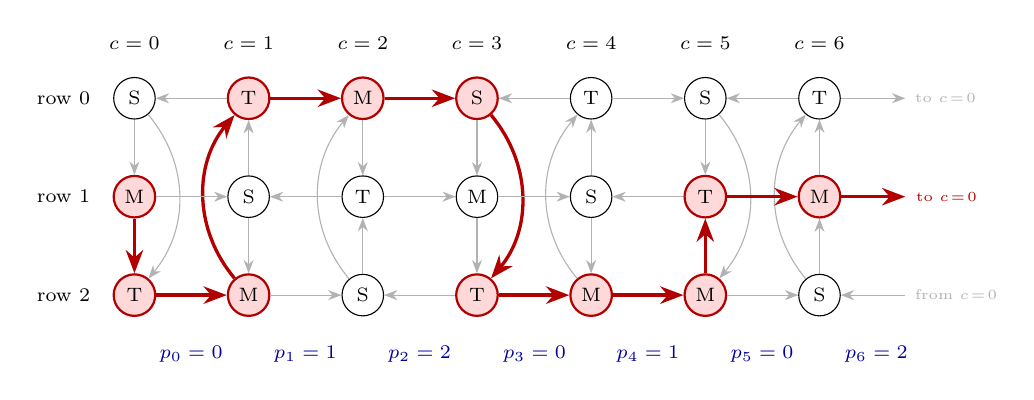
\begin{tikzpicture}[>=Stealth,v/.style={circle,draw,inner sep=1.2pt,minimum size=15pt,font=\scriptsize}]
\node[v] (v00) at (0.00,0.00) {S};
\node[v,fill=red!15,draw=red!70!black,thick] (v10) at (0.00,-1.25) {M};
\node[v,fill=red!15,draw=red!70!black,thick] (v20) at (0.00,-2.50) {T};
\node[font=\scriptsize] at (0.00,0.7) {$c=0$};
\node[font=\scriptsize,text=blue!60!black] at (0.72,-3.25) {$p_0=0$};
\node[v,fill=red!15,draw=red!70!black,thick] (v01) at (1.45,0.00) {T};
\node[v] (v11) at (1.45,-1.25) {S};
\node[v,fill=red!15,draw=red!70!black,thick] (v21) at (1.45,-2.50) {M};
\node[font=\scriptsize] at (1.45,0.7) {$c=1$};
\node[font=\scriptsize,text=blue!60!black] at (2.17,-3.25) {$p_1=1$};
\node[v,fill=red!15,draw=red!70!black,thick] (v02) at (2.90,0.00) {M};
\node[v] (v12) at (2.90,-1.25) {T};
\node[v] (v22) at (2.90,-2.50) {S};
\node[font=\scriptsize] at (2.90,0.7) {$c=2$};
\node[font=\scriptsize,text=blue!60!black] at (3.62,-3.25) {$p_2=2$};
\node[v,fill=red!15,draw=red!70!black,thick] (v03) at (4.35,0.00) {S};
\node[v] (v13) at (4.35,-1.25) {M};
\node[v,fill=red!15,draw=red!70!black,thick] (v23) at (4.35,-2.50) {T};
\node[font=\scriptsize] at (4.35,0.7) {$c=3$};
\node[font=\scriptsize,text=blue!60!black] at (5.08,-3.25) {$p_3=0$};
\node[v] (v04) at (5.80,0.00) {T};
\node[v] (v14) at (5.80,-1.25) {S};
\node[v,fill=red!15,draw=red!70!black,thick] (v24) at (5.80,-2.50) {M};
\node[font=\scriptsize] at (5.80,0.7) {$c=4$};
\node[font=\scriptsize,text=blue!60!black] at (6.52,-3.25) {$p_4=1$};
\node[v] (v05) at (7.25,0.00) {S};
\node[v,fill=red!15,draw=red!70!black,thick] (v15) at (7.25,-1.25) {T};
\node[v,fill=red!15,draw=red!70!black,thick] (v25) at (7.25,-2.50) {M};
\node[font=\scriptsize] at (7.25,0.7) {$c=5$};
\node[font=\scriptsize,text=blue!60!black] at (7.97,-3.25) {$p_5=0$};
\node[v] (v06) at (8.70,0.00) {T};
\node[v,fill=red!15,draw=red!70!black,thick] (v16) at (8.70,-1.25) {M};
\node[v] (v26) at (8.70,-2.50) {S};
\node[font=\scriptsize] at (8.70,0.7) {$c=6$};
\node[font=\scriptsize,text=blue!60!black] at (9.42,-3.25) {$p_6=2$};
\draw[->,gray!60] (v00) to (v10);
\draw[->,gray!60,bend left=40] (v00) to (v20);
\draw[->,red!70!black,very thick] (v10) to (v20);
\draw[->,gray!60] (v11) to (v21);
\draw[->,gray!60] (v11) to (v01);
\draw[->,red!70!black,very thick,bend left=40] (v21) to (v01);
\draw[->,gray!60,bend left=40] (v22) to (v02);
\draw[->,gray!60] (v22) to (v12);
\draw[->,gray!60] (v02) to (v12);
\draw[->,gray!60] (v03) to (v13);
\draw[->,red!70!black,very thick,bend left=40] (v03) to (v23);
\draw[->,gray!60] (v13) to (v23);
\draw[->,gray!60] (v14) to (v24);
\draw[->,gray!60] (v14) to (v04);
\draw[->,gray!60,bend left=40] (v24) to (v04);
\draw[->,gray!60,bend left=40] (v05) to (v25);
\draw[->,gray!60] (v05) to (v15);
\draw[->,red!70!black,very thick] (v25) to (v15);
\draw[->,gray!60] (v26) to (v16);
\draw[->,gray!60,bend left=40] (v26) to (v06);
\draw[->,gray!60] (v16) to (v06);
\draw[->,gray!60] (v01) -- (v00);
\draw[->,gray!60] (v10) -- (v11);
\draw[->,red!70!black,very thick] (v20) -- (v21);
\draw[->,red!70!black,very thick] (v01) -- (v02);
\draw[->,gray!60] (v12) -- (v11);
\draw[->,gray!60] (v21) -- (v22);
\draw[->,red!70!black,very thick] (v02) -- (v03);
\draw[->,gray!60] (v12) -- (v13);
\draw[->,gray!60] (v23) -- (v22);
\draw[->,gray!60] (v04) -- (v03);
\draw[->,gray!60] (v13) -- (v14);
\draw[->,red!70!black,very thick] (v23) -- (v24);
\draw[->,gray!60] (v04) -- (v05);
\draw[->,gray!60] (v15) -- (v14);
\draw[->,red!70!black,very thick] (v24) -- (v25);
\draw[->,gray!60] (v06) -- (v05);
\draw[->,red!70!black,very thick] (v15) -- (v16);
\draw[->,gray!60] (v25) -- (v26);
\draw[->,gray!60] (v06) -- (9.79,0.00) node[right,font=\tiny]{to $c\!=\!0$};
\draw[->,red!70!black,very thick] (v16) -- (9.79,-1.25) node[right,font=\tiny]{to $c\!=\!0$};
\draw[<-,gray!60] (v26) -- (9.79,-2.50) node[right,font=\tiny]{from $c\!=\!0$};
\node[font=\scriptsize] at (-0.90,0.00) {row 0};
\node[font=\scriptsize] at (-0.90,-1.25) {row 1};
\node[font=\scriptsize] at (-0.90,-2.50) {row 2};
\end{tikzpicture}}
\caption{$n=7$, $p=(0,1,2,0,1,0,2)$, column labels show $S,M,T$. The gadget is at $c=2$;
the highlighted induced directed cycle has length $11$ (row arcs leaving column $6$
wrap to column $0$).}
\end{figure}

\begin{corollary}
For odd $n$ with $3\nmid n$, no admissible orientation of $C_3\square C_n$ is
kernel-perfect. For odd $n$ with $3\mid n$, the only possible ones are the $12$ Latin
orientations ($p_c=p_0\pm c$, two choices of $\varepsilon$, three of $p_0$).
\end{corollary}

\section{The Latin orientations are kernel-perfect (computer-assisted)}

\begin{theorem}\label{thm:if}
For every odd $k$, the $12$ Latin orientations of $C_3\square C_{3k}$ are kernel-perfect.
Hence the kernel method proves $C_3\square C_{3k}$ is $3$-choosable.
\end{theorem}

\begin{proof}[Method]
Kernel existence in an induced subdigraph $H$ is checked column by column with a
$20$-state automaton: the state after column $c$ records the kernel vertex of column $c$
(at most one, since columns are cliques) and which present vertices of column $c$ still
need absorbing through a row arc to column $c+1$. Every $H$ is a choice of present rows
in each column; one period of $3$ columns gives $8^3$ boolean $20\times20$ block matrices,
and $H$ on $C_3\square C_{3k}$ has a kernel iff the product of its $k$ blocks has a
nonzero boolean trace. We computed, for each of the $12$ orientations, the complete set
of pairs (product, parity of $k$) closed under multiplication by blocks ($1515$ or $1604$
pairs). No product with $k$ odd has zero trace, which proves the claim for every odd $k$.
\end{proof}

\paragraph{Checks.} The automaton agreed with direct kernel search on $37{,}800$ induced
subdigraphs. Independently, all $2^{27}$ induced subdigraphs of each Latin orientation of
$C_3\square C_9$ were checked by brute force. For even $k$ the claim fails: on
$C_3\square C_6$ there is a $9$-vertex kernel-less induced subdigraph, found by both
methods.

\begin{theorem}[Summary for $m=3$]
For odd $n\ge3$, $C_3\square C_n$ has a kernel-perfect orientation with $\Delta^+\le2$ if
and only if $3\mid n$, and then exactly $12$.
\end{theorem}

\section{\texorpdfstring{$m\ge5$}{m >= 5}}

\begin{proposition}[computer-verified]
$C_5\square C_5$ has no kernel-perfect admissible orientation: all $143{,}224$ admissible
orientations contain an induced odd directed cycle.
\end{proposition}
Lifting the $C_3\square C_3$ Latin orientations in both coordinates also fails: all $12$
lifts to $C_9\square C_9$ contain induced odd directed cycles.

\begin{conjecture}
For odd $m,n\ge5$, $C_m\square C_n$ has no kernel-perfect orientation with $\Delta^+\le2$.
\end{conjecture}

\section{Related verified facts}

\begin{itemize}[leftmargin=1.4em]
\item \textbf{Edge deletion, exact.} For $C_5\square C_5$ and $C_5\square C_7$, every
coefficient $[x_w\prod_{v\ne w}x_v^2]\,P_{G-e}$ with $w$ off the cycle of $e$ was computed
over $\mathbb F_{1000003}$ (Laso\'n / Karasev--Petrov formula with cube roots of unity)
and is nonzero, hence nonzero over $\mathbb Z$. So, as for $m=3$, any bad $3$-list
assignment of these graphs has $L(u)\cap L(v)\ne\emptyset$ on every edge.
\item \textbf{Independent check of the $m=3$ coefficient formulas} (Theorem 1 of
``Deleting one edge\ldots''): all values agree for $n=3,5,7,9$.
\item \textbf{List-colouring search.} No bad $3$-list assignment of $C_3\square C_5$ exists
with a palette of $4$ colours (SAT search, exhaustive); larger palettes and
$C_5\square C_5$ still running.
\end{itemize}

\end{document}
